\anonsection{Введение}
\label{sec:0_vvedenie} \index{0_vvedenie}

В современных вычислительных системах, особенно во встраиваемых и высокопроизводительных приложениях, критически важным ресурсом часто является оперативная память. При выполнении набора работ (задач), связанных отношением частичного порядка (граф потока данных), каждая работа может порождать один или несколько выходных буферов, которые занимают память до момента, когда все их потребители завершат выполнение. Ограниченность памяти накладывает дополнительные условия на допустимость расписания: в любой момент времени суммарный объём активных буферов не должен превышать заданного предела $M$. Требуется построить такое расписание (распределение работ по процессорам и порядок их выполнения), чтобы общая длительность (makespan) была минимальной.

Данная задача возникает, например, при проектировании систем цифровой обработки сигналов (ЦОС), где каждый вычислительный модуль (например, БПФ, фильтр) потребляет и производит массивы данных фиксированного размера, а память является ограничивающим фактором~\cite{Ershov1962}. Аналогичные проблемы характерны для научных конвейерных вычислений (scientific workflows), где промежуточные результаты могут иметь большой объём~\cite{BalashovBasalov2025}. Многопроцессорное планирование с учётом ограничений памяти является NP-трудной задачей, поэтому практические методы делятся на две категории: точные (например, сведение к целочисленному линейному программированию) и приближённые (например, жадные эвристики).

В работе~\cite{Savitsky2023} предложен жадный алгоритм для многопроцессорного списочного планирования с ограничением на долю межпроцессорных передач; в настоящей работе этот алгоритм адаптирован для учёта памяти, а также разработана новая эвристика STS (Smallest Time Space), учитывающая не только длительность работы, но и объём создаваемых ею буферов и длительности потребителей. Для малых графов (до 21 вершины) выполнено сведение к задаче ЦЛП по схеме, аналогичной описанной в работе~\cite{Senyushkina2025} для однопроцессорного случая, с добавлением переменных, моделирующих пересечение интервалов активности буферов. Выбор решателя SCIP обоснован в~\cite{Senyushkina2025}.

На рис.~\ref{fig:graph_example} приведён пример графа работ, а на~\ref{fig:shed_example} - двух возможных расписаний (построенных жадным алгоритмом и оптимального). Видно, что оптимальное расписание позволяет лучше использовать память и процессоры, избегая длительных простоев.\\

Для описанной выше задачи в работе представлены и исследованы жадные алгоритмы с двумя различными эвристиками, а также подход на основе целочисленного линейного программирования.\\

\begin{figure}[h]
	\centering
	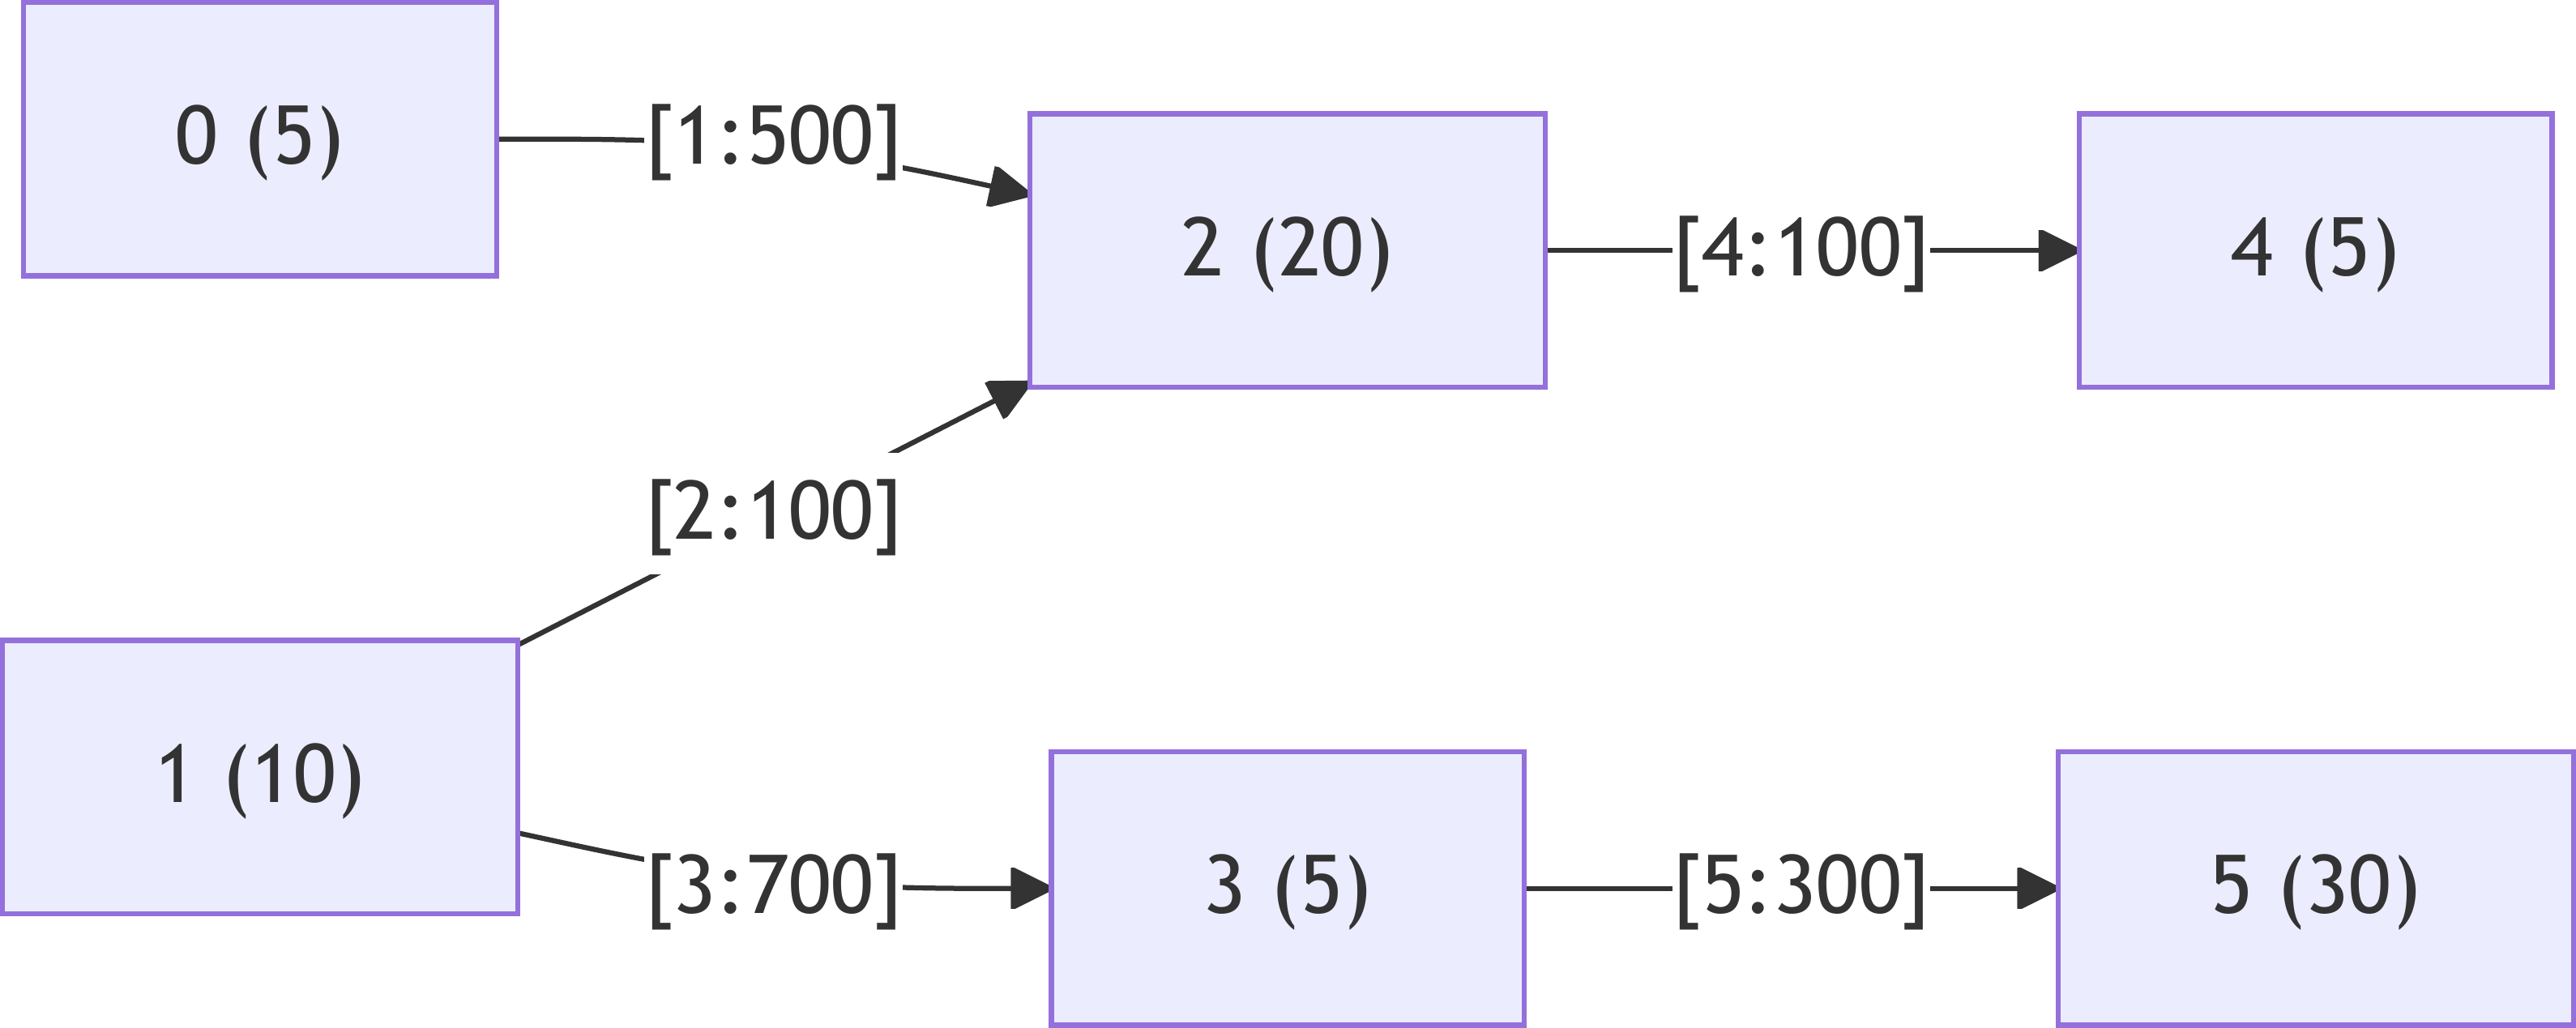
\includegraphics[width=1\textwidth]{pictures/g6-1.png}
	\caption{}
	\label{fig:graph_example}
\end{figure}

\begin{figure}[h]
	\centering
	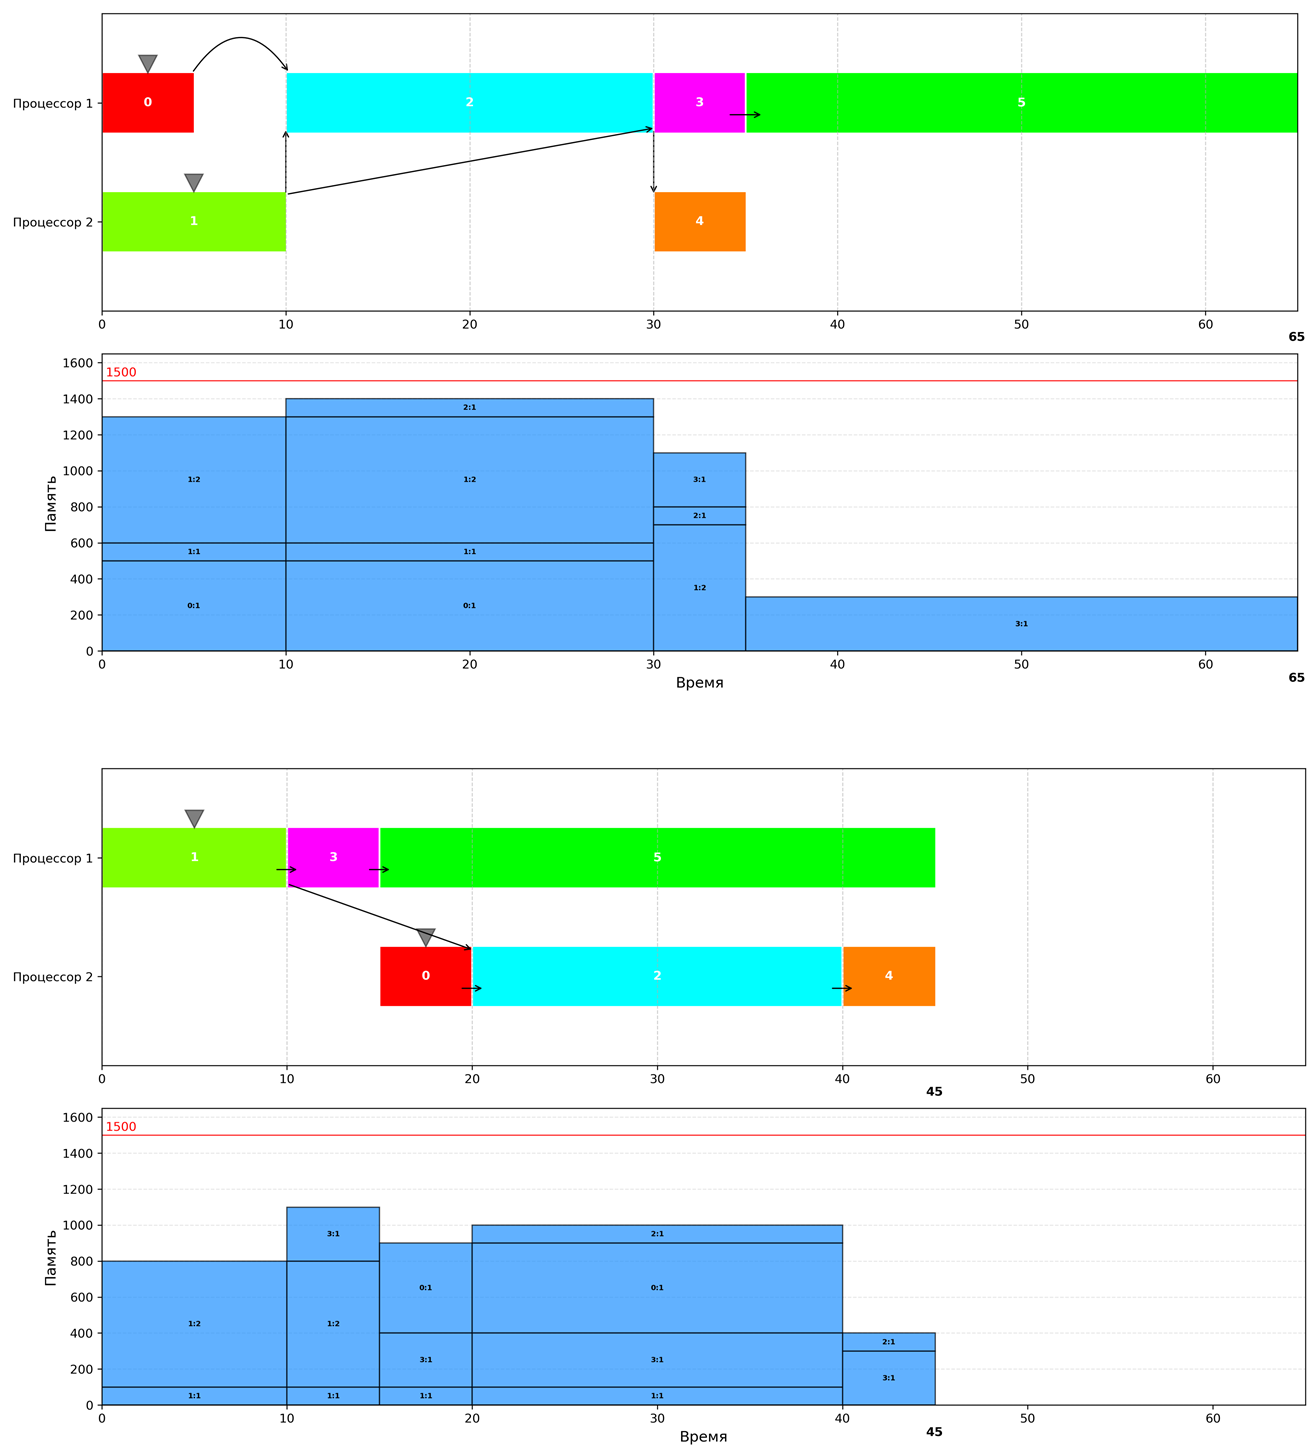
\includegraphics[width=1\textwidth]{pictures/intro2.png}
	\caption{сверху - ЖА с EFT, снизу - ЛП}
	\label{fig:shed_example}
\end{figure}